\documentclass[12pt]{article}
\usepackage[utf8]{inputenc}
\usepackage{hyperref}
\usepackage{tikz}


\title{Representing Numbers}
\author{Shaan Fulton}
\date{\today}

\begin{document}

\maketitle

\section*{Unsigned Numbers Are Easy}

We use a sequence of bits and the idea of a positional number system to create a bijection between any set of characters and our simple binary transistors. Because our array of bits is just a base-2 number system, it already represents numbers. However, there are some considerations to keep in mind when thinking of how to represent negative numbers in such a way that we can easily perform hardware computation on them.


\subsection*{Summation with Bits}

We can easily implement a summation operation on two unsigned binary numbers.

\begin{center}
\begin{tabular}{cccccc}
    & 1 & 1 & 0 & 1 \\[-1pt]
  + & 1 & 0 & 1 & 1 \\ \hline
carry: & 1 & 1 & 1 & 0 & \\[-1pt]
sum: & 1 & 1 & 0 & 0 & 0 \\
\end{tabular}
\end{center}

\section*{Unsigned Numbers Are Harder}

But what about negative numbers? An intuitive method of representing negatives is deciding that the left leading bit will represent our sign. A 1 might correlate to a negative signed number, and a 0 might correlate to a positive signed number.

\begin{center}
\begin{tabular}{|c|c|c|c|}
    \hline
    \textbf{Sign Bit} & \textbf{Magnitude Bits} & \textbf{Full Binary ($0b$)} & \textbf{Value} \\
    \hline
    0 & 101 & 0b0101 & $+5$ (positive) \\
    1 & 101 & 0b1101 & $-5$ (negative) \\
    \hline
\end{tabular}
\end{center}

This is the sign-magnitude encoding for numbers. It is terrible for numerical operations. Try to add two sign-magnitude numbers and you'll see why: the result makes no sense because as the magnitude digits of a sign magnitude number increases, the actual value represented may be decreasing or increasing depending on the sign. Thus it is totally incompatible with our simple summation operation described above.

\subsection*{Two's Complement and Biased Encodings}

We present two alternatives to the sign-magnitude approach that are beautifully compatible with our simple summation operation. This is critical, as it makes building the hardware summation operation much simpler.

The \textbf{two's complement} approach is as follows:


\begin{enumerate}
    \item \textbf{Check the leftmost bit (sign bit):}
    \begin{itemize}
        \item If it is \texttt{0}, the number is positive. Read it as a normal binary number.
        \item If it is \texttt{1}, the number is negative.
    \end{itemize}
    \item \textbf{If the number is negative (sign bit is 1):}
    \begin{enumerate}
        \item Imagine that you invert (flip) all the bits (change \texttt{0} to \texttt{1} and \texttt{1} to \texttt{0}).
        \item Add 1 to the result.
        \item The answer is the magnitude, but the number is negative.
    \end{enumerate}
\end{enumerate}

\noindent
\textit{Why is this useful?} Two's complement allows positive and negative numbers to be added and subtracted using the same binary addition rules. There are not two ways to write zero (as with sign-magnitude), and the ordering of numbers is continuous—making math operations simpler for computers.

\begin{center}
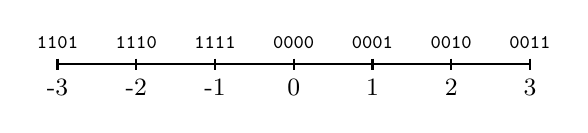
\begin{tikzpicture}[x=1cm, y=0.7cm]
    % Draw the number line
    \draw[thick] (-3,0) -- (3,0);
    % Tick marks and labels
    \foreach \x/\b in {-3/1101, -2/1110, -1/1111, 0/0000, 1/0001, 2/0010, 3/0011} {
        \draw[thick] (\x,0.1) -- (\x,-0.1);
        \node[below] at (\x,-0.1) {\small \x};
        \node[above] at (\x,0.1) {\scriptsize \texttt{\b}};
    }
\end{tikzpicture}
\end{center}

\textbf{Biased encoding} is even simpler. The idea is we just use unsigned numbers, however, we shift them as we need to. So we might create an encoding with a bias of 127. \texttt{0b00000000}, or binary 0, is now -127. We can go all the way up to positive 127, \texttt{0b11111111}. All summation operations work perfectly.

\subsection*{Encoding Summary}

\begin{itemize}
\item{Sign-Magnitude: Never used, problematic for numerical operations}
\item{Two's Complement: Standard for \texttt{int}
\item{Biased Encoding: Manually implemented on top of \texttt{uint}}
\end{itemize}

\end{document}

